% fig2-architecture.tex — Figure 2: Sego core architecture (English)
% Subsystems follow the repository structure (cf. deepwiki.com/007M7/Sego-Agent)
% Layout uses positioning chains only — node sizes adapt to content (no truncation).
\documentclass[tikz,border=10pt]{standalone}
\usetikzlibrary{arrows.meta,positioning,fit,backgrounds,calc}

\begin{document}
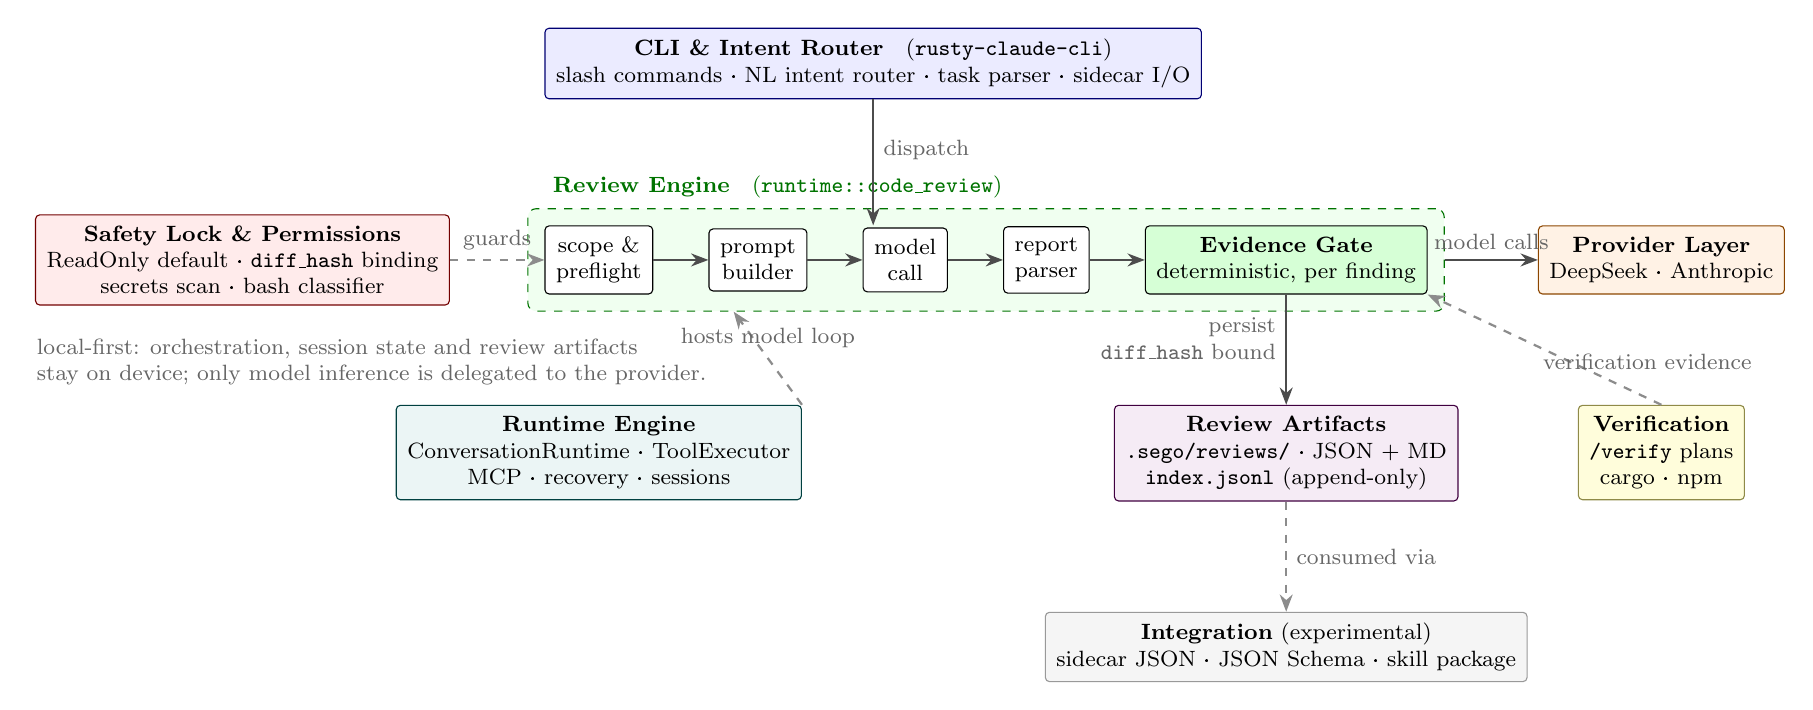
\begin{tikzpicture}[
  font=\small,
  comp/.style={draw, rounded corners=1.5pt, fill=white, font=\footnotesize,
               align=center, inner sep=4pt},
  sys/.style={comp, align=center},
  arr/.style={-{Stealth[length=2.2mm]}, thick, draw=black!70},
  darr/.style={-{Stealth[length=2.2mm]}, thick, draw=black!45, dashed},
  lab/.style={font=\footnotesize, text=black!60},
  grp/.style={draw=black!15, dashed, rounded corners=3pt, inner sep=6pt}
]

% ================= Row 1: CLI =================
\node[sys, fill=blue!8, draw=blue!45!black] (cli)
  {\textbf{CLI \& Intent Router} \; (\texttt{rusty-claude-cli})\\
   \footnotesize slash commands · NL intent router · task parser · sidecar I/O};

% ================= Row 2: Review Engine pipeline =================
\node[comp, below left=16mm and 0mm of cli.south west, anchor=north west] (pre)  {scope \&\\ preflight};
\node[comp, right=7mm of pre]  (prompt) {prompt\\ builder};
\node[comp, right=7mm of prompt] (mcall) {model\\ call};
\node[comp, right=7mm of mcall] (parse) {report\\ parser};
\node[comp, right=7mm of parse, fill=green!16] (gate) {\textbf{Evidence Gate}\\ deterministic, per finding};

\begin{scope}[on background layer]
  \node[grp, fill=green!6, draw=green!45!black] (rebox) at (0,0)
    [fit=(pre)(gate)] {};
\end{scope}
\node[lab, text=green!45!black, anchor=south west]
  at ([xshift=2mm]rebox.north west)
  {\textbf{Review Engine} \; (\texttt{runtime::code\_review})};
\draw[arr] (pre) -- (prompt);
\draw[arr] (prompt) -- (mcall);
\draw[arr] (mcall) -- (parse);
\draw[arr] (parse) -- (gate);
\draw[arr] (cli.south) -- node[lab, right, pos=0.4] {dispatch} (pre.north -| cli.south |- pre.north);

% ================= Row 2 sides =================
\node[sys, fill=red!8, draw=red!45!black, left=12mm of pre] (safety)
  {\textbf{Safety Lock \& Permissions}\\ \footnotesize ReadOnly default · \texttt{diff\_hash} binding\\ \footnotesize secrets scan · bash classifier};
\draw[darr] (safety.east) -- node[lab, above, pos=0.5] {guards} (pre.west);

\node[sys, fill=orange!10, draw=orange!55!black, right=14mm of gate] (prov)
  {\textbf{Provider Layer}\\ \footnotesize DeepSeek · Anthropic};
\draw[arr] (rebox.east) -- node[lab, above, pos=0.5] {model calls} (prov.west);

% ================= Row 3 =================
\node[sys, fill=teal!8, draw=teal!50!black, below=14mm of pre] (runtime)
  {\textbf{Runtime Engine}\\ \footnotesize ConversationRuntime · ToolExecutor\\ \footnotesize MCP · recovery · sessions};
\node[sys, fill=violet!8, draw=violet!50!black, below=14mm of gate] (art)
  {\textbf{Review Artifacts}\\ \footnotesize \texttt{.sego/reviews/} · JSON + MD\\ \footnotesize \texttt{index.jsonl} (append-only)};
\node[sys, fill=yellow!14, draw=yellow!50!black, below=14mm of prov] (verif)
  {\textbf{Verification}\\ \footnotesize \texttt{/verify} plans\\ \footnotesize cargo · npm};

\draw[arr] (gate.south) -- node[lab, left, pos=0.4, align=right] {persist\\ \footnotesize \texttt{diff\_hash} bound} (art.north);
\draw[darr] (runtime.north east) -- node[lab, above, pos=0.5] {hosts model loop} ($(rebox.south west)!0.45!(rebox.south)$);
\draw[darr] (verif.north) -- node[lab, below right, pos=0.55] {verification evidence} (gate.south east);

% ================= Row 4: Integration =================
\node[sys, fill=black!4, draw=black!40, below=14mm of art] (integ)
  {\textbf{Integration} \footnotesize(experimental)\\ \footnotesize sidecar JSON · JSON Schema · skill package};
\draw[darr] (art.south) -- node[lab, right, pos=0.5] {consumed via} (integ.north);

% ================= Side note =================
\node[lab, anchor=north west, align=left] at ($(safety.south west)+(-1mm,-3mm)$)
  {local-first: orchestration, session state and review artifacts\\
   stay on device; only model inference is delegated to the provider.};

\end{tikzpicture}
\end{document}
